\documentclass[a4paper,10pt]{article}
\usepackage{fullpage}
\usepackage{float}
\usepackage[english]{babel}
\usepackage{graphicx,subfig,wrapfig}
\usepackage{amsmath,amsfonts,amsthm,amssymb}
\usepackage{fancyhdr,fancybox,color}
\usepackage{enumerate}
\usepackage[amssymb]{SIunits}
\definecolor{MyBlue}{rgb}{0,0.3,0.6}
\usepackage[colorlinks=true,
            linkcolor=MyBlue,
            plainpages=false,
            citecolor=MyBlue,
            urlcolor=MyBlue]{hyperref}
\usepackage[all]{hypcap}
\usepackage[url=false,
backend=bibtex,
style=authoryear-comp,
doi=true,
isbn=true,
backref=false,
dashed=false,
maxcitenames=2,
maxbibnames=99,
natbib=true]{biblatex}
\addbibresource{refrence.bib}

\nonfrenchspacing
\begin{document}
\noindent Chair: Physics of Fluids group
\begin{center}
 \begin{LARGE}
  Bubble in volcanoes: Numerics
 \end{LARGE}
\end{center}

\section*{Project description}
Bubbles play an essential role in magmatic and mud volcanoes. It has been shown that the growth, motion, and burst of the bubbles at the interface of the conduit control the eruption (see Figure~\ref{Figure::Typical}). In this project, we aim to understand more about the role of bubbles in volcanoes. In particular, we will study the burst of bubbles at the liquid-gas interface that is believed to control the eruption.\\
In our simulation, we will use an in-house developed read-to-use code to solve the problem of the bubble bursting at the surface of magma. We will ignore heat-transfer at this stage and focus on the hydrodynamics of the process. We will use a Non-Newtonian model to mimic the properties of magma or mud.

\begin{figure}[H]
\begin{center}
 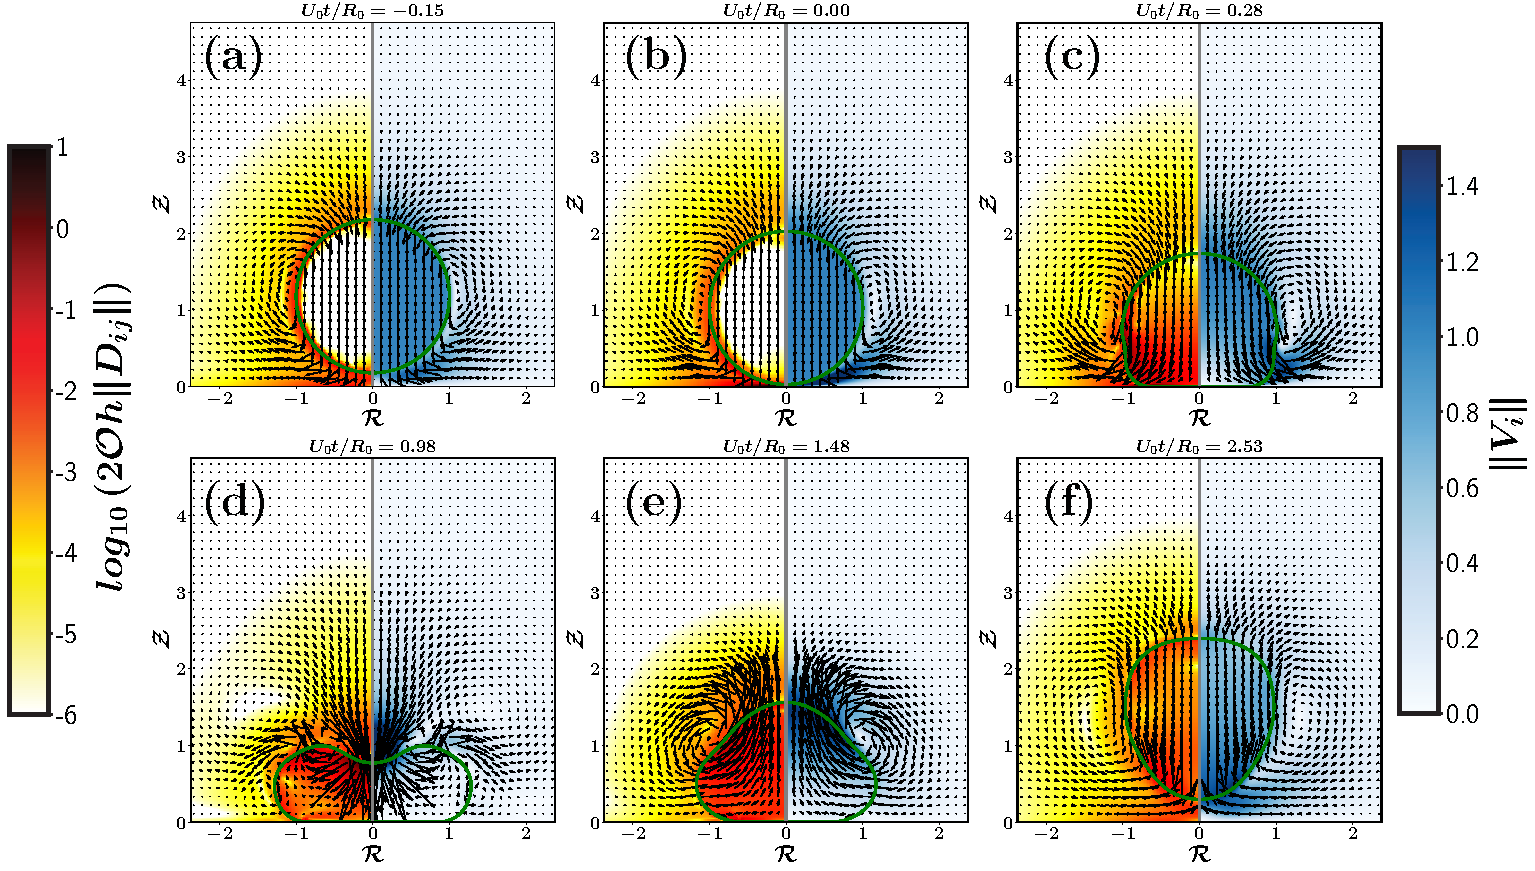
\includegraphics[width=0.9\textwidth]{Figure1}
 \caption{A schematic showing the role of bubbles in a volcanic eruption (on the left,  \cite{gonnermann2007fluid}). The simulation of the collapse of the cavity formed by bursting of bubbles at the magma-air interface (on the right).}
 \label{Figure::Typical}
\end{center}
\end{figure}

\section*{What are the learning components?}
Learning expectations primarily focus on familiarity with the state-of-the-art simulation code, Basilisk C.\\

\noindent Specifically, the intern will learn

\begin{enumerate}
	\item volume of fluid (VoF) numerical simulation using Basilisk C to model non-Newtonian flows.
	\item modeling and analyzing exotic and complex flows involving multi-physics and multi-scale. 
	\item connecting computer based simulations to real-life geophysical flows in volcanoes. 
\end{enumerate}

\noindent {\it Soft skills:}

\noindent After from the above-mentioned technical skills, the intern will also develop a range of soft skills. The internship will not only expose them to learn crucial research techniques but also give them a foreign exposure. At the end of the internship, they will have a knack to work effectively with other people from various ethnic, educational, and work experience backgrounds. This will help them later in the undergraduate studies as well as get a Ph.D. position at a distinguished group.

\section*{What will the intern do?}
In the Physics of Fluids group, we are looking for enthusiastic students to join our newly established projects on fluid mechanics of volcanoes, in collaboration with the fluidlab at University of Amsterdam.

\begin{enumerate}
\itemsep0em
\item They will learn about fundamental geophysical fluid mechanics and bubble dynamics.
\item They will work with experimentalists and numericists. 
\item They will work with the Computational Fluid Dynamics (CFD) fundamentals, and use the free software program Basilisk C \href{http://basilisk.dalembert.upmc.fr}{(http://basilisk.dalembert.upmc.fr)}.
\item They will learn how to do basic and advance data analysis. 
\end{enumerate}

\section*{Future perspectives}

The training period will help develop substantive knowledge in dynamics of bubbles and will strengthen the fundamentals of direct numerical simulations. The Physics of Fluids chair at the University of Twente hosts one of the biggest international personnel (including Ph.D. students and postdocs) and has a strong reputation at an international stage. The intern will be introduced to how research is conducted and evaluated in the area of droplet phenomenon. The intern will also learn to demonstrate their ability to communicate the result of his research in an efficient manner. These essential skills will give them an exposure to doctoral research and will be helpful for him to pursue doctoral studies after graduation.


\section*{Project timeline}
\begin{figure}[H]
	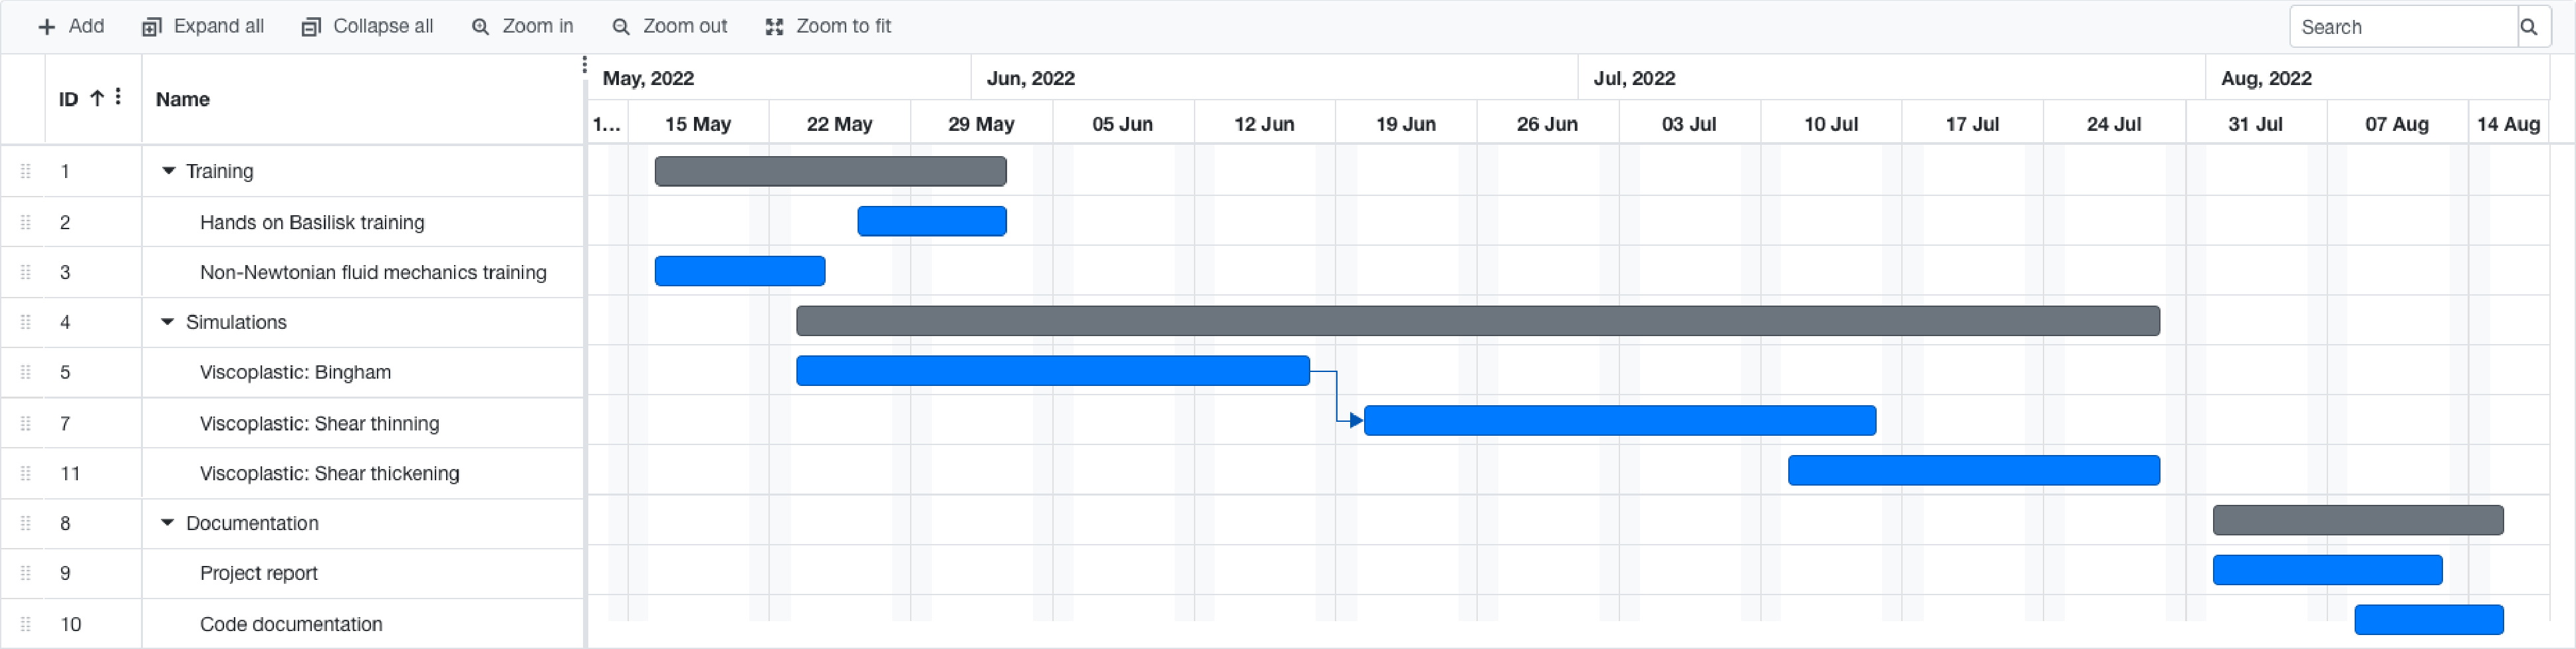
\includegraphics[width=\textwidth]{OnlineGantt2022045.pdf}
	\caption{Timeline and trainee program}
\end{figure}

\section*{Host personnel}
If you have any questions, fell free to contact  Vatsal Sanjay (details below).

\begin{center}
\begin{tabular}{|l|l|l|l|}
\hline \textbf{Supervision} & \textbf{E-mail} & \textbf{Tel.}  & \textbf{Office} \\
\hline Vatsal Sanjay & \href{mailto:contact@vatsalsanjay.com}{contact@vatsalsanjay.com} & +31 687668747/+91 7895940240 &  UT \\
\hline Dr. Maziyar Jalaal   & \href{mailto:m.jalaal@uva.nl}{m.jalaal@uva.nl}& & UvA \\
\hline Dr. Uddalok Sen   & \href{mailto:u.sen@utwente.nl}{u.sen@utwente.nl}& +31 53 489 9064  & UT \\
\hline Prof. D. Lohse & \href{mailto:d.lohse@utwente.nl}{d.lohse@utwente.nl} & +31 53 489 8076 & UT  \\
\hline
\end{tabular}
\end{center}

\pagebreak

\vspace{20mm}

\noindent Sign: \hrulefill

\hspace*{0mm}\phantom{Sign: }Mahashay Jee.

\hspace*{0mm}\phantom{Sign: }Intern

\vspace{20mm}

\noindent
Sign: \hrulefill

\hspace*{0mm}\phantom{Sign: }Vatsal Sanjay.

\hspace*{0mm}\phantom{Sign: }Daily supervisor

\vspace{20mm}

\noindent
Sign: \hrulefill

\hspace*{0mm}\phantom{Sign: }prof. dr. Detlef Lohse.

\hspace*{0mm}\phantom{Sign: }Chair, Physics of Fluids, University of Twente

\vspace{20mm}
\noindent
Sign: \hrulefill

\hspace*{0mm}\phantom{Sign: }Name:

\hspace*{0mm}\phantom{Sign: }Home Institution:
\vspace{15mm}

\printbibliography
\end{document}
